\documentclass[article,11pt,a4paper,brazil]{abntex2}

\usepackage{lmodern}
\usepackage[T1]{fontenc}
\usepackage[utf8]{inputenc}
\usepackage{indentfirst}
\usepackage{nomencl}
\usepackage{color}
\usepackage{graphicx}
\usepackage{microtype}
\usepackage{listings}
\usepackage{float}
\usepackage{multirow}
\usepackage{amsmath}
\renewcommand*{\insertchapterspace}{%
	\addtocontents{lof}{\protect\addvspace{10pt}}%
	\addtocontents{lot}{\protect\addvspace{10pt}}}

% ---
% Pacotes fundamentais 
% ---
\usepackage{lmodern}			% Usa a fonte Latin Modern
\usepackage[T1]{fontenc}		% Selecao de codigos de fonte.
\usepackage[utf8]{inputenc}		% Codificacao do documento (conversão automática dos acentos)
\usepackage{indentfirst}		% Indenta o primeiro parágrafo de cada seção.
\usepackage{nomencl} 			% Lista de simbolos
\usepackage{color}				% Controle das cores
\usepackage{graphicx}			% Inclusão de gráficos
\usepackage{microtype} 			% para melhorias de justificação
\usepackage{array}
% Pacotes adicionais, usados apenas no âmbito do Modelo Canônico do abnteX2
% ---
\usepackage{lipsum}				% para geração de dummy text
% ---
\lstdefinestyle{mystyle}{
	backgroundcolor=\color{backcolour},   
	commentstyle=\color{codegreen},
	keywordstyle=\color{magenta},
	numberstyle=\tiny\color{codegray},
	stringstyle=\color{codepurple},
	basicstyle=\ttfamily\footnotesize,
	breakatwhitespace=false,         
	breaklines=true,                 
	captionpos=b,                    
	keepspaces=true,                 
	numbers=left,                    
	numbersep=5pt,                  
	showspaces=false,                
	showstringspaces=false,
	showtabs=false,                  
	tabsize=2
}
\lstset{frame=tb,
	language=python,
	aboveskip=3mm,
	belowskip=3mm,
	showstringspaces=false,
	columns=flexible,
	basicstyle={\small\ttfamily},
	numbers=none,
	numberstyle=\tiny\color{gray},
	keywordstyle=\color{blue},
	commentstyle=\color{dkgreen},
	stringstyle=\color{mauve},
	breaklines=true,
	breakatwhitespace=true
	tabsize=3
}


% --- Informações de dados para CAPA e FOLHA DE ROSTO ---
\titulo{Modelagem Estatística de Doenças Cardiovasculares com Base em Dados Clínicos}
\tituloestrangeiro{Statistical Modelling of Cardiovascular Diseases Based on Clinical Data}

\autor{
	Iara Cristina Mescua Castro }

\data{\today}
% ---

% ---
% Configurações de aparência do PDF final

% alterando o aspecto da cor azul
\definecolor{blue}{RGB}{41,5,195}

% informações do PDF
\makeatletter

\hypersetup{
	%pagebackref=true,
	pdftitle={\@title}, 
	pdfauthor={\@author},
	pdfsubject={Modelo de artigo científico com abnTeX2},
	pdfcreator={LaTeX with abnTeX2},
	pdfkeywords={abnt}{latex}{abntex}{abntex2}{atigo científico}, 
	colorlinks=true,       		% false: boxed links; true: colored links
	linkcolor=blue,          	% color of internal links
	citecolor=blue,        		% color of links to bibliography
	filecolor=magenta,      		% color of file links
	urlcolor=blue,
	bookmarksdepth=4
}
\makeatother
% --- 

% ---
% compila o indice
% ---
\makeindex
% ---

% ---
% Altera as margens padrões
% ---
\setlrmarginsandblock{3cm}{3cm}{*}
\setulmarginsandblock{3cm}{3cm}{*}
\checkandfixthelayout
% ---


% --- 
% Espaçamentos entre linhas e parágrafos 
% --- 

% O tamanho do parágrafo é dado por:
\setlength{\parindent}{1.3cm}

% Controle do espaçamento entre um parágrafo e outro:
\setlength{\parskip}{0.2cm}  % tente também \onelineskip

% Espaçamento simples
\SingleSpacing


% ----
% Início do documento
% ----
\begin{document}
	
	% Seleciona o idioma do documento (conforme pacotes do babel)
	%\selectlanguage{english}
	\selectlanguage{brazil}
	
	% Retira espaço extra obsoleto entre as frases.
	\frenchspacing 
	
	% ----------------------------------------------------------
	% ELEMENTOS PRÉ-TEXTUAIS
	% ----------------------------------------------------------
	
	%---
	%
	% Se desejar escrever o artigo em duas colunas, descomente a linha abaixo
	% e a linha com o texto ``FIM DE ARTIGO EM DUAS COLUNAS''.
	% \twocolumn[    		% INICIO DE ARTIGO EM DUAS COLUNAS
	%
	%---
	
	% página de titulo principal (obrigatório)
	\maketitle
	\thispagestyle{empty}
	\begin{citacao}
		Estudo de caso da disciplina de Modelagem Estatística submetido como trabalho da A2 no 5° período de Matemática Aplicada.\\
		Professor: Luiz Max
	\end{citacao}
	% titulo em outro idioma (opcional)

\newpage
\thispagestyle{empty}

%\newpage	

%\thispagestyle{empty}
	% resumo em português
	
\begin{resumoumacoluna}
		O objetivo do trabalho é desenvolver um modelo estatístico para prever a ocorrência de doenças cardiovasculares com base em dados reais de pacientes e elaborar uma análise exploratória dos dados (EAD), com o intuito de identificar possíveis relações entre as covariáveis do dataset que podem vir a influenciar um indivíduo a contrair doenças cardiovasculares. O conjunto utilizado está disponível no [Kaggle](https://www.kaggle.com/sulianova/cardiovascular-disease-dataset), que contém 70.000 registros de pacientes, com 12 variáveis de entrada e 1 variável de saída, que indica se o paciente possui ou não doença cardiovascular. 
		
		\vspace{\onelineskip}
		
		\noindent
		\textbf{Palavras-chave}: modelagem. estatística. doença cardiovascular. saúde. análise de dados. regressão linear. bayes. aprendizado de máquinas. R
\end{resumoumacoluna}
	
%\newpage	
%\thispagestyle{empty}
	% resumo em inglês
	\renewcommand{\resumoname}{Abstract}
	\begin{resumoumacoluna}
		\begin{otherlanguage*}{english}
			The objective of this work is to develop a statistical model to predict the occurrence of cardiovascular diseases based on real patient data and to elaborate an exploratory data analysis (EDA), in order to identify possible relationships between the covariates of the dataset that may influence an individual to contract cardiovascular diseases. The dataset used is available on [Kaggle](https://www.kaggle.com/sulianova/cardiovascular-disease-dataset), which contains 70,000 patient records, with 12 input variables and 1 output variable, which indicates whether the patient has cardiovascular disease or not.
			
			\vspace{\onelineskip}
			
			\noindent
			\textbf{Keywords}: modeling. statistics. cardiovascular disease. healthcare. data analysis. linear regression. bayes. machine learning. R.
		\end{otherlanguage*}  
	\end{resumoumacoluna}

	\newpage

	\thispagestyle{empty}
	\tableofcontents*
	\newpage

	\section{Introdução}
	\setcounter{page}{1}
	\pagestyle{plain}
	Doenças cardiovasculares são a principal causa de morte no mundo. Segundo a Organização Mundial da Saúde (OMS) \cite{who-cardiovascular-diseases}, 17,9 milhões de pessoas morreram em 2019 devido a doenças cardiovasculares, sendo que 85\% dessas mortes são causadas por infarto do miocárdio e acidente vascular cerebral (AVC). A OMS e a Organização Pan-Americana de saúde \cite{opas-doenças-cardiovasculares} também estimam que 80\% das mortes prematuras por doenças cardiovasculares podem ser evitadas com mudanças no estilo de vida, como: evitar o consumo de tabaco, alimentação saudável e prática de atividades físicas. 
	
	A análise de dados clínicos é um componente fundamental da epidemiologia e medicina baseada em evidências. Ela permite que pesquisadores e médicos compreendam a complexa dinâmica das doenças, assim como os fatores que influenciam a sua ocorrência e a eficácia das intervenções. No caso das doenças cardiovasculares, a situação é especialmente relevante devido à sua prevalência e mortalidade associada, fazendo da análise desses dados uma atividade de grande importância para a saúde pública.
	
	Diante dessa situação, iremos trabalhar com um dataset composto por 70.000 registros coletados em exames médicos na plataforma \textit{Kaggle} \cite{datasetcardiovascular}, uma plataforma que disponibiliza publicação e coleta de conjunto de dados aos seus usuários. Nele, há 12 características sobre cada paciente e a variável "alvo" que representa a presença ou não de uma doença cardiovascular. As características foram separadas em 3 inputs:
	
	\noindent $\cdot$ Objetiva: Informação factual.\\
	$\cdot$ Exame: Resultados de exames médicos.\\
	$\cdot$ Subjetiva: Informação dada pelo paciente.
	

	\begin{table}[H]
		\caption{Variáveis do Dataset}
		\centering
		\begin{tabular}{|c|c|c|p{8cm}|}
			\hline
			Variáveis & Input & Tipo & \multicolumn{1}{c|}{Descrição}\\
			\hline
			\hline
			id &  - & Num. Contínuo & ID do registro\\
			\hline
			age & objetiva & Num. Contínuo & Idade (em dias)\\
			\hline
			height & objetiva & Num. Contínuo & Altura (em metros)\\
			\hline
			weight & objetiva & Num. Contínuo & Peso (em kg.)\\
			\hline
			gender & objetiva & Num. Contínuo & Sexo, valor 1 para mulher e 2 para homem\\
			\hline
			ap\_hi & objetiva & Num. Contínuo & Pressão Sistólica\\
			\hline
			ap\_ho & exame & Num. Contínuo & Pressão Diastólica\\
			\hline
			cholesterol & exame & Categórica Ord. & Nível de Colesterol, Valor 1 para normal,
			2 para acima do normal e 3 para bem acima do normal\\
			\hline
			gluc & exame & Categórica Ord. & Nível da Glicose, Valor 1 para normal, 2 para acima do normal e 3 para bem acima do normal\\
			\hline
			smoke & subjetiva & Categórica Bin. & Se é fumante, Valor 0 para não fumante e 1 para fumante\\
			\hline
			alco & subjetiva & Categórica Bin. & Se ingere álcool, Valor 0 se não ingere e 1 se ingere\\
			\hline
			active & subjetiva & Categórica Bin. & Se pratica atividade física, Valor 0 se pratica e 1 se não pratica\\ 
			\hline 
			cardio & alvo & Categórica Bin. & Informa a presença ou não de doença cardiovascular. Valor 0 se não tem e 1 se tem\\
			\hline
		\end{tabular}
		\label{table:variaveis}
	\end{table}

	\newpage
	Variáveis como idade, altura, peso e gênero são características demográficas e biológicas fundamentais que podem influenciar o risco de doenças cardiovasculares. Já variáveis de saúde como pressão sistólica (ap\_hi), pressão diastólica (ap\_lo), colesterol e glicose são medidas clínicas diretas do estado de saúde cardiovascular de um indivíduo. E por fim, o consumo de tabaco (smoke), consumo de álcool (alco) e a atividade física (active) são fatores comportamentais que terão suas relações com a saúde cardiovascular exploradas mais a fundo. 
	
	O principal objetivo é desenvolver um modelo de regressão logística que possa ajudar a detectar se uma pessoa corre o risco de adquirir uma doença cardiovascular. Informar a probabilidade de um paciente ter ou desenvolver uma doença cardiovascular desempenha um papel fundamental na tomada de decisões médicas. Além disso, eles também podem ajudar a identificar indivíduos em risco que ainda não foram diagnosticados, o que poderia resultar em uma intervenção mais precoce e, portanto, melhores resultados para os pacientes com redução do risco. 
	
	Segundo a OMS, vidas poderiam ser salvas por meio de melhorias no acesso à saúde, sobretudo no que diz respeito ao controle da pressão alta, do colesterol alto e de outras condições que aumentam o risco de doenças cardiovasculares. Então, a análise destes dados pode aumentar nossa compreensão dos fatores que contribuem para essas condições, o que poderia levar a melhores estratégias de prevenção e controle.
	
	O artigo será dividido partes. No Capítulo 2 será apresentada a metodologia utilizada para a construção de modelos. No Capítulo 3 serão analisados os dados para construção da análise exploratória (AED), ajustes do modelo, e também serão apresentados as estimativas e predições obtidas. E por fim, no capítulo 4 será elaborada a conclusão com considerações finais sobre os classificadores e uma discussão das limitações metodológicas e limitações do dataset, assim como o caminho para possíveis trabalhos futuros.
	\section{Metodologia}
	\subsection{Tratamento dos Dados}
	A fase inicial de qualquer projeto de análise de dados envolve a preparação e limpeza dos dados, processos essenciais para garantir a integridade e a qualidade dos dados coletados. Neste estudo, apesar de não haverem valores nulos (Nan), realizamos várias transformações e seleções em nosso conjunto de dados.
	
	\noindent $\boldsymbol{\cdot}$ A idade dos participantes em \textit{age}, que originalmente estava registrada em dias, foi convertida para anos para facilitar a interpretação. Esse ajuste é importante pois permite uma compreensão mais intuitiva da variável e facilita a interpretação dos resultados.
	
	\noindent $\boldsymbol{\cdot}$ O gênero dos participantes em \textit{gender}, inicialmente registrado como 'um' e 'dois', foi transformado em variáveis binárias. Nós codificamos 'um' como 0 e 'dois' como 1, convertendo a variável categórica nominal em uma variável categórica ordinal. 
	
	\noindent $\boldsymbol{\cdot}$ Criamos a variável \textit{IMC} (Índice de Massa Corporal), calculada a partir das colunas peso e altura. O IMC é uma métrica comumente usada para categorizar o status de peso dos indivíduos e tem sido associado a diversos resultados de saúde.
	
	\noindent $\boldsymbol{\cdot}$ Transformamos os valores negativos de \textit{ap\_hi} e \textit{ap\_lo} em valores absolutos para corrigir possíveis erros de entrada de dados. A pressão arterial não pode ser negativa, então assumimos que esses valores foram erros de digitação. 
	
	\noindent $\boldsymbol{\cdot}$ Removemos registros que caíam fora dos intervalos clinicamente plausíveis para a pressão arterial. Eliminamos aqueles com pressão sistólica abaixo de 60 ou acima de 250 e pressão diastólica abaixo de 30 ou acima de 200. Adicionalmente, removemos dados onde a pressão sistólica era menor ou igual à pressão diastólica, já que isso é fisiologicamente impossível.
	
	\noindent $\boldsymbol{\cdot}$ Descartamos registros com pesos abaixo de 30 kg ou altura superior a 220 cm, bem como IMCs menores que 10 ou maiores que 55, para garantir que nossos dados representassem uma população clinicamente relevante.
	
	\subsection{Modelos Categóricos/Binários}
	
	Modelos categóricos (ou binários) são métodos de análise de dados amplamente utilizados em situações em que a variável de resposta de interesse tem apenas duas categorias possíveis. Nestes modelos, as variáveis de resposta são frequentemente codificadas como 0 e 1, onde 1 indica a presença de um determinado atributo (por exemplo, uma doença) e 0 sua ausência. Em nosso caso, a variável de resposta é a presença ou ausência de doenças cardiovasculares, que é binária.
	
	Esses modelos são particularmente úteis para a análise de dados em pesquisa médica e de saúde, onde muitas vezes estamos interessados em entender os fatores que influenciam a ocorrência de uma doença. O modelo categórico/binário permite que investiguemos a relação entre essa variável de resposta binária e um conjunto de variáveis explicativas, que podem ser tanto contínuas quanto categóricas. 
	
	As variáveis contínuas no nosso caso incluem idade, altura, peso, pressão arterial sistólica e diastólica, enquanto as variáveis categóricas incluem gênero, colesterol, glicose, tabagismo, consumo de álcool e atividade física.
	
	\subsection{Modelo Generalizado Linear (GLM) e Distribuição Binomial}
	
	Optamos por utilizar um Modelo Generalizado Linear (GLM) para a nossa análise, com uma distribuição binomial para a nossa variável de resposta categórica/binária. O GLM é uma extensão dos Modelos Lineares Simples que permitem que a variável de resposta siga qualquer distribuição da família exponencial, que inclui distribuições normal, binomial, poisson, gama, entre outras. 
	
	A distribuição binomial é adequada para a nossa análise porque a nossa variável de resposta, a presença ou ausência de doenças cardiovasculares, é uma variável binária e a distribuição binomial modela o número de sucessos em um número fixo de tentativas independentes, cada uma com a mesma probabilidade de sucesso. Neste caso, cada "tentativa" corresponde a um paciente no nosso conjunto de dados.
	
	Para ajustar o GLM, usamos a função \textit{glm()} em R, que permite especificar a distribuição e a função de ligação do modelo. A função de ligação logit, que é o padrão para a distribuição binomial, relaciona a variável de resposta com as variáveis explicativas de uma maneira que garante que as estimativas de probabilidade estejam entre 0 e 1. 
	
	Além disso, as funções básicas do R se destacaram na análise, visto que usamos a função \textit{summary()} para visualizar os coeficientes e informações do modelo, a função \textit{predict()} para fazer previsões.
	
	\subsection{Odds Ratio e Interpretação de Coeficientes}
	
	Para interpretar os coeficientes de um modelo de regressão logística, usualmente calculamos o odds ratio, que é obtido aplicando a função exponencial aos coeficientes. O odds ratio pode ser interpretado como a mudança nas chances (odds) de um evento (neste caso, ter uma doença cardiovascular) para cada unidade de mudança na variável preditora, mantendo todas as outras variáveis constantes.
	
	Para calcular as odds ratios e os intervalos de confiança, utilizamos a biblioteca \textit{broom} em R. Além disso, também calculamos os p-valores para cada coeficiente. Os p-valores nos ajudam a determinar se a variável independente tem uma relação estatisticamente significativa com a variável dependente. Se o p-valor é menor que o nível de significância (geralmente 0.05), podemos rejeitar a hipótese nula de que o coeficiente é igual a zero, o que significa que a variável tem um efeito significativo na variável de resposta.
	
	\subsection{Avaliação do Modelo}
	Para avaliar a qualidade do nosso modelo, utilizamos várias métricas. Começando pelo Critério de Informação de Akaike (AIC), o Critério de Informação Bayesiano (BIC), e o Critério de Informação Corrigido de Akaike (AICC). Essas métricas nos permitem comparar modelos diferentes e escolher o modelo que tem o melhor equilíbrio entre ajuste aos dados e complexidade do modelo \cite{brewer2016relative}.
	
	 O AIC é baseado em duas partes: a probabilidade dos dados, dada uma estimativa dos parâmetros do modelo, e a complexidade do modelo (número de parâmetros). O BIC é semelhante ao AIC, mas adiciona um termo de penalidade maior para modelos com mais parâmetros. O AICC é uma versão corrigida do AIC que leva em conta o tamanho da amostra e é particularmente útil quando a relação entre o número de observações e o número de parâmetros é pequena. Em todos esses critérios, um valor menor indica um melhor equilíbrio entre ajuste aos dados e complexidade do modelo. 
	
	Também calculamos a matriz de confusão \cite{wiki-confusion-matrix}, uma tabela que resume o desempenho de um algoritmo de classificação. Os elementos da diagonal principal da matriz de confusão correspondem às observações corretamente classificadas, enquanto os outros elementos indicam os erros. 
	
	\begin{itemize}
	\item Verdadeiro Positivo (VP): Quando o classificador prevê uma amostra como positiva e ela é realmente positiva.
	\item  Falso Positivo (FP): Quando o classificador prevê uma amostra como positiva, mas na verdade ela é negativa.
	\item  Falso Positivo (VN): Quando o classificador prevê como uma amostra negativa e realmente é negativo.
	\item  Falso Positivo (FN): Quando o classificador prevê uma amostra como negativa, mas na verdade ela é positiva.
	\end{itemize}
	
	\begin{tabular}{|c|c|c|c|}
		\multicolumn{2}{c|}{} & \multicolumn{2}{c|}{Classes Reais} \\
		\multicolumn{2}{c|}{} & Positivo (1) & Negativo (0) \\
		\hline
		\multirow{2}{*}{Classes previstas} & Positivo (1) & VP & FP \\
		\cline{3-4}
		& Negativo (0) & FN & VN \\
		\hline
	\end{tabular}	
\newpage

	\noindent A \textbf{acurácia} mede a proporção total de previsões corretas, enquanto a precisão mede a proporção de previsões positivas que são realmente positivas. 	
	$$
	\text { acurácia }=\frac{\text { Número de predições corretas }}{\text { todas as predições }}=\frac{V P+V N}{V P+F P+V N+F N}
	$$	
	\noindent A \textbf{precisão} é a proporção de previsões positivas que são realmente positivas 
	$$
	\text { precisão }=\frac{V P}{V P+F P}
	$$
	O \textbf{recall} mede a proporção de casos positivos que foram corretamente identificados, e o f1-score é uma média harmônica da precisão e recall.
	$$
	\text { recall }=\frac{V P}{V P+F N}
	$$
	O \textbf{$F_1$-score} é a média harmônica da precisão e recall. Enquanto a média regular trata igualmente todos os valores, a média harmônica dá muito mais peso aos valores mais baixos. Como resultado, o classificador só obterá uma $F_1$-score alta se a recall e a precisão forem altas (GÉRON, 2019).
	$$
	F_1 \text {-score }=2 * \frac{\text { precisão } * \text { recall }}{\text { precisão } +\text { recall }}=\frac{V P}{V P+\frac{F N+F P}{2}}
	$$

	Finalmente, criamos curvas ROC (Receiver Operating Characteristic) com o pacote \textit{pRoc} e calculamos a área sob a curva (AUC) para avaliar o desempenho do modelo em diferentes limiares de classificação. A AUC é uma métrica útil para avaliar o desempenho geral do modelo, independente do limiar de classificação escolhido.
	\newpage
	\section{Resultados}
	\subsection{Análise Exploratória de Dados (AED)}
	Antes de ajustar nosso modelo, realizamos uma Análise Exploratória de Dados (AED) em Python para obter uma compreensão mais profunda dos nossos dados e selecionar covariáveis de interesse. Com o pacote "Seaborn", ela fornece uma visão inicial sobre as distribuições dos dados, as relações entre as variáveis, e possíveis anomalias.
	
	Começamos nossa AED com um scatter plot entre as variáveis de idade, altura, peso, pressão arterial sistólica (\textit{ap\_hi}) e pressão arterial diastólica (\textit{ap\_lo}). Esses gráficos nos ajudam a visualizar as relações entre as variáveis e a presença de doenças cardiovasculares após o tratamento do dataset na Seção 2.1.
	
	\begin{figure}[H]
		\centering
		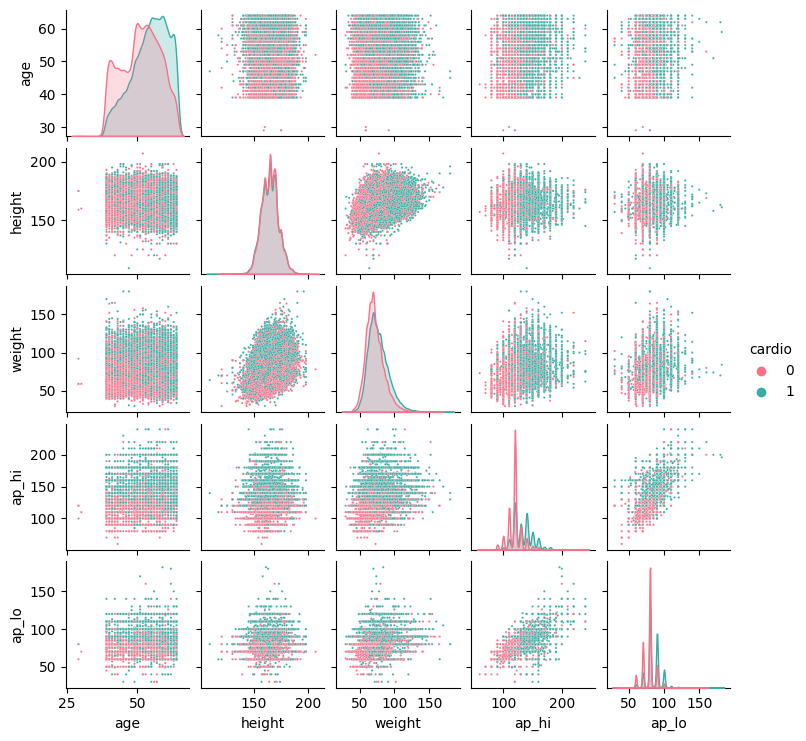
\includegraphics[width=0.8\linewidth]{Images/pairplot.png}
	\end{figure}
	
	Já começamos a notar uma distinção entre os valores 0 e 1 na maioria das relações, exceto em \textit{height}. A seguir, analisamos as quantidades de pacientes que fumam, consomem álcool e praticam atividades físicas, segmentadas pela presença e ausência de doenças cardiovasculares. Esses gráficos de contagem nos permitem observar a distribuição desses fatores de risco em pacientes com e sem doenças cardiovasculares.
	
	\begin{figure}[H]
		\centering
		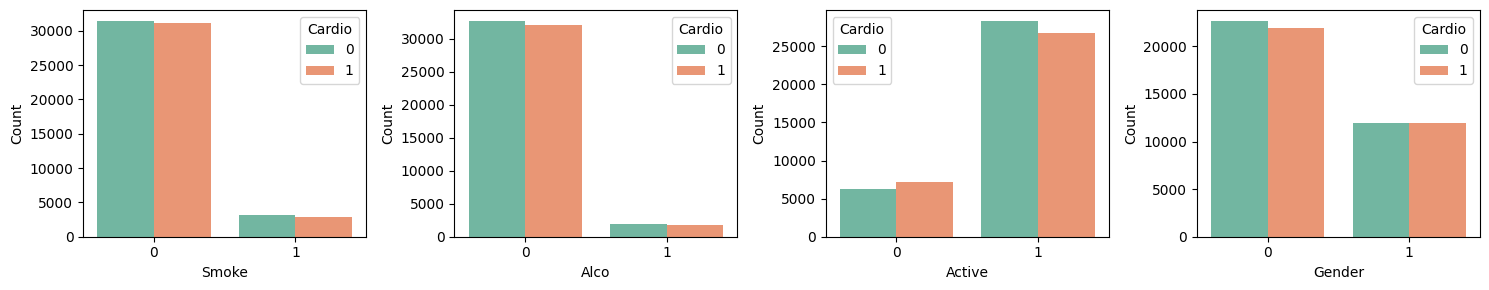
\includegraphics[width=1\linewidth]{Images/categorical1.png}
	\end{figure}
	
	Podemos ver que em todos as quantias são bem próximas, com uma leve diferença para pacientes que não tem uma doença cardiovascular quando não fumam, não bebem e praticam exercício físico, respectivamente. Da mesma forma, examinamos os níveis de colesterol e glucose para pacientes com e sem doenças cardiovasculares.	
	\begin{figure}[H]
		\centering
		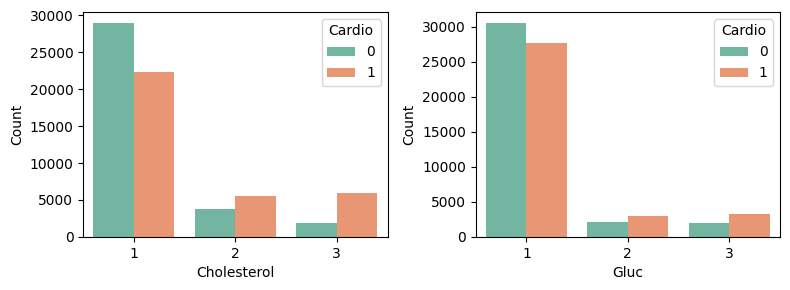
\includegraphics[width=0.6\linewidth]{Images/categorical2.png}
	\end{figure}	
	As diferenças são mais acentuadas, níveis elevados de colesterol e glucose estão mais presentes em pacientes com doenças cardiovasculares, especialmente para "bem acima do normal".
	
	 Em seguida, visualizamos a distribuição da idade dos pacientes e do Índice de Massa Corporal (IMC), separados pela presença ou ausência de doenças cardiovasculares. A idade é um importante fator de risco para doenças cardiovasculares, e o IMC é um indicador comum da saúde geral de um indivíduo.
	
	\begin{figure}[H]
		\centering
		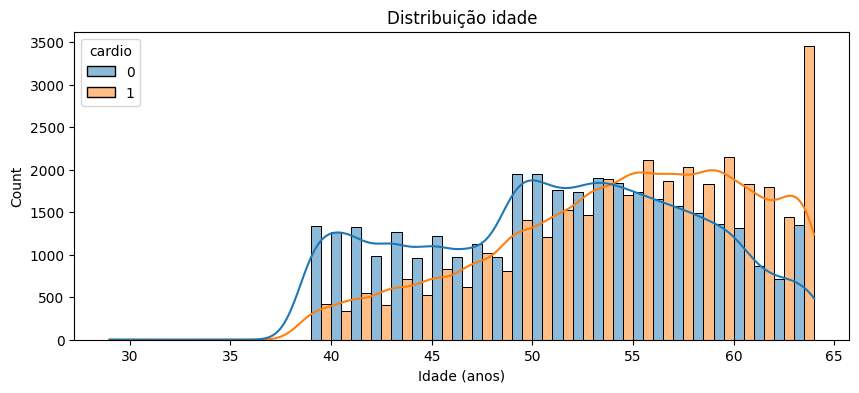
\includegraphics[width=0.8\linewidth]{Images/dist_idade.png}
	\end{figure}
	\begin{figure}[H]
		\centering
		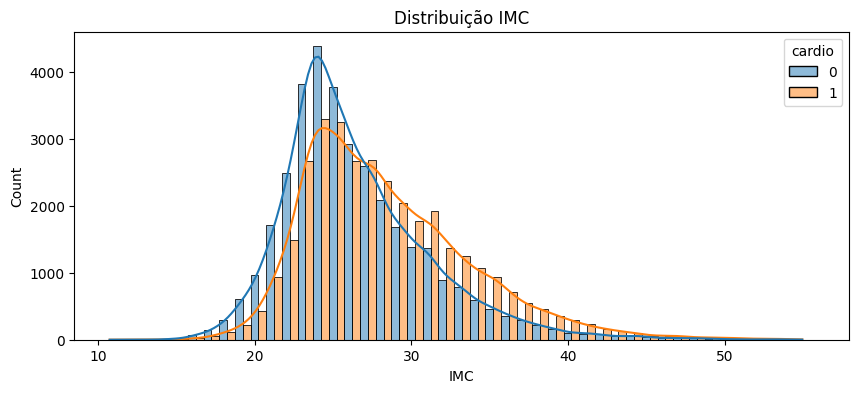
\includegraphics[width=0.8\linewidth]{Images/dist_imc.png}
	\end{figure}
	
	Podemos ver que a partir dos 55 anos e 28 de IMC, doenças cardiovasculares passam a ser parte da maioria dos pacientes e tendem a aumentar.
	
	Analisamos os box plots das variáveis numéricas: pressão sanguínea sistólica, diastólica, peso e altura, para pacientes com e sem doenças cardiovasculares. Esses gráficos nos permitem identificar diferenças nas distribuições dessas variáveis entre os grupos de pacientes.
	\begin{figure}[H]
		\centering
		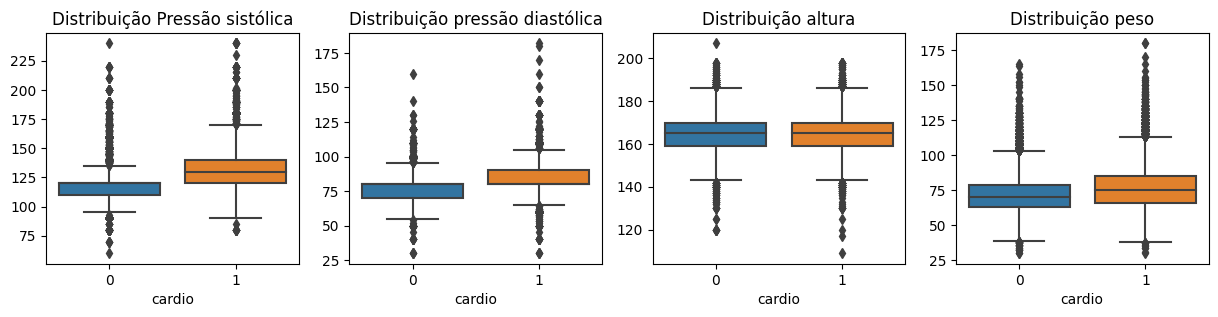
\includegraphics[width=1\linewidth]{Images/boxplots.png}
	\end{figure}
	
	Novamente, a pressão sistólica e diastólica se ressaltaram. Por último, calculamos e visualizamos uma matriz de correlação entre as variáveis. Esta etapa é crucial para identificar colinearidades potenciais que podem influenciar o ajuste do nosso modelo.
	\begin{figure}[H]
		\centering
		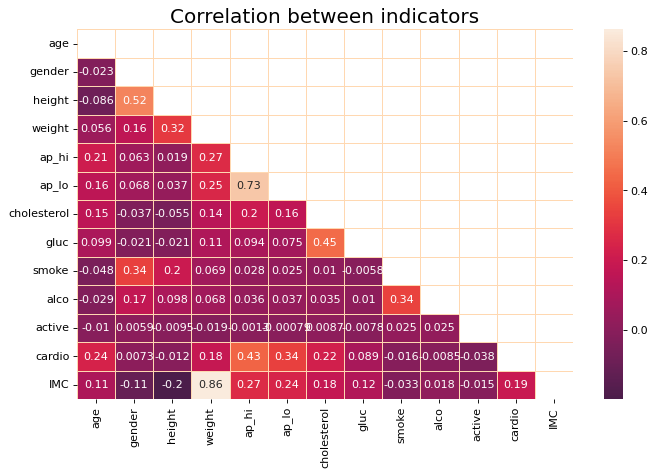
\includegraphics[width=0.75\linewidth]{Images/corr.png}
	\end{figure}
	
	\subsection{Modelos Finais}
	Como foi dito na Seção 2.3, o modelo de regressão foi ajustado em R, utilizando a biblioteca padrão:
	\begin{lstlisting}[language=R]
model1 <- glm(cardio ~ age + weight + gender + height + IMC + ap_hi + ap_lo + cholesterol + gluc + smoke + alco + active,data = train, family = binomial)
	\end{lstlisting}
Dispensamos \textit{height} e \textit{gender} que não se destacaram na AED. Tal como o IMC que não teve * no summary() do Modelo 1.
	\begin{lstlisting}[language=R]
model2 <- glm(cardio ~ age + weight + ap_hi + ap_lo + cholesterol + gluc + smoke + alco + active, data = train, family = binomial)
	\end{lstlisting}
	\subsection{Odds-Ratio}
	\noindent Para calcular o Odds-Ratio, basta calcular a exponencial dos coeficientes.
	\begin{lstlisting}[language=R]
coefficients1 <- coef(model1)	
odds_ratios1 <- exp(coefficients1)
	
coefficients2 <- coef(model2)	
odds_ratios2 <- exp(coefficients2)
	\end{lstlisting}
	As tabelas a seguir mostra os Odds-Ratios para cada variável nos modelos 1 e 2. Por exemplo, no modelo 1, um aumento de uma unidade no IMC está associado a um aumento de 1,0169928946 nas odds de ter uma doença cardiovascular, mantendo constantes todas as outras variáveis.
	
	Modelo 1:
\[
\begin{array}{rrrrrr}
	\text {(Intercept)} & \text {age} & \text {weight} & \text {gender} & \text {height} & \text {IMC} \\
	0.0001124234 & \text {NA} & 1.0055539248 & 1.0329447817 & 0.9962756880 & 1.0179538372 \\
	\text{ap\_hi} & \text{ap\_lo} & \text{cholesterol} & \text{gluc} & \text{smoke} & \text{alco} \\
	1.0601147675 & 1.0123568328 & 1.7372350411 & 0.9093902358 & 0.8175683701 & 0.8077217851 \\
	\text{active} \\
	0.8127675883 
\end{array}
\]
	Modelo 2:
\[
\begin{array}{rrrrrr}
	\text{(Intercept)} & \text{age} & \text{weight} & \text{gender} & \text{ap\_hi}\\
	6.569469 \times 10^{-5} & \text{NA} & 1.010766 \times 10^{0} & 9.592586 \times 10^{-1} & 1.060526 \times 10^{0} \\ 
	\text{cholesterol} & \text{gluc} & \text{smoke} & \text{alco} & \text{active} & \\
	1.748292 \times 10^{0} & 9.099134 \times 10^{-1} & 8.130558 \times 10^{-1} & 8.081532 \times 10^{-1} & 8.144292 \times 10^{-1} \\
 \text{ap\_lo}\\
  1.012288 \times 10^{0} 
 
\end{array}
\]
	\subsection{Métricas de Performance}
	Esta sub-seção descreve a avaliação de desempenho para os modelos com as medidas de Verdadeiro Positivo (TP), Verdadeiro Negativo (TN), Falso Positivo (FP), Falso Negativo (FN), F-score. Daí, obtemos as seguintes medidas:
	
	\begin{center}
		\begin{tabular}{|c|c|c|}
		\hline
		\textbf{Métricas} & \textbf{Modelo 1} & \textbf{Modelo 2} \\
		\hline
		Accuracy & 0.7192795 & 0.7190368 \\
		Precision & 0.6454253 & 0.6453279 \\
		Recall & 0.7555606 & 0.7551881 \\
		F1 Score & 0.696164 & 0.6959491 \\
		\hline
	\end{tabular}
	\end{center}
	
	\subsection{P-valores}
	\noindent P-valores das covariáveis, calculadas com a função tidy():
	\begin{lstlisting}[language=R]
tidy(model1)
tidy(model2)
	\end{lstlisting}
	\begin{figure}[H]
		\centering
		\begin{minipage}[b]{0.4\textwidth}
			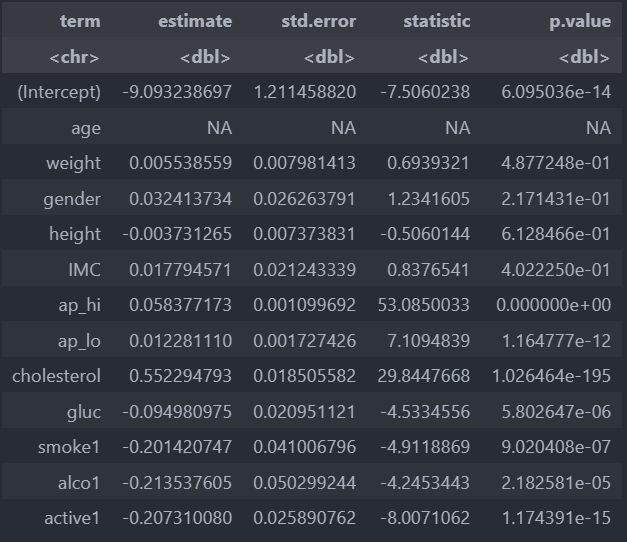
\includegraphics[width=\textwidth]{Images/pvalue1.png}
			\caption{Modelo 1}
		\end{minipage}
		\hspace{2mm}
		\begin{minipage}[b]{0.4\textwidth}
			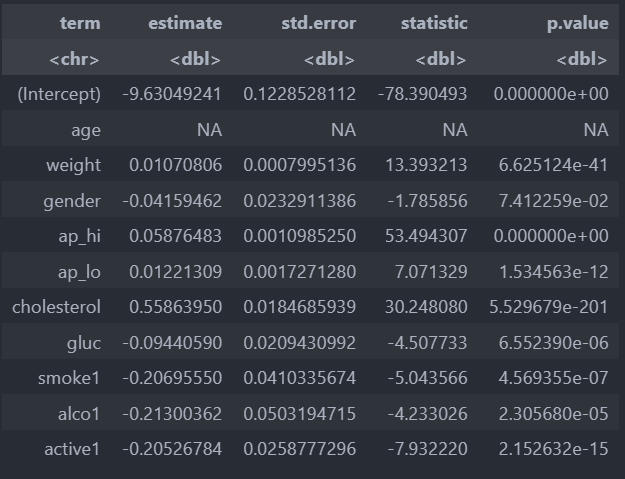
\includegraphics[width=\textwidth]{Images/pvalue2.png}
			\caption{Modelo 2}
		\end{minipage}
	\end{figure}
	\subsection{Intervalos de Confiança}
	\noindent Intervalo de confiança de 95\% com a função \textit{confint()} dos Modelos 1 e 2, respectivamente.
	\begin{center}
		\begin{minipage}{0.45\textwidth}
			\centering
			\begin{tabular}{rrr} 
				& $2.5\%$ & $97.5\%$ \\
				\hline
				(Intercept) & -11.468978038 & -6.71971018 \\
				age & $\mathrm{NA}$ & $\mathrm{NA}$ \\
				weight & -0.010104337 & 0.02118592 \\
				gender & -0.019070481 & 0.08388417 \\
				height & -0.018185972 & 0.01072158 \\
				IMC & -0.023831590 & 0.05945140 \\
				ap\_hi & 0.056229646 & 0.06054054 \\
				ap\_lo & 0.008895148 & 0.01566684 \\
				cholesterol & 0.516107545 & 0.58865149 \\
				gluc & -0.136072717 & -0.05394130 \\
				smoke1 & -0.281858721 & -0.12110638 \\
				alco1 & -0.312211100 & -0.11502527 \\
				active1 & -0.258060292 & -0.15656750 \\
			\end{tabular}
		\end{minipage}
		\hfill
		\begin{minipage}{0.45\textwidth}
			\centering
			\begin{tabular}{rrr} 
				& $2.5\%$ & $97.5\%$ \\
				\hline
				(Intercept) & -9.872154534 & -9.390564575 \\
				age & $\mathrm{NA}$ & $\mathrm{NA}$ \\
				weight & 0.009142334 & 0.012276476 \\
				gender & -0.087256906 & 0.004044688 \\
				ap\_hi & 0.056619603 & 0.060925920 \\
				ap\_lo & 0.008827728 & 0.015598246 \\
				cholesterol & 0.522525363 & 0.594924307 \\
				gluc & -0.135481670 & -0.053381687 \\
				smoke1 & -0.287445753 & -0.126588530 \\
				alco1 & -0.311717422 & -0.114452299 \\
				active1 & -0.255992477 & -0.154550776 \\
			\end{tabular}
		\end{minipage}
	\end{center}
	\subsection{AUC e Roc Curves}
	\begin{figure}[H]
		\centering
		\begin{minipage}[b]{0.35\textwidth}
			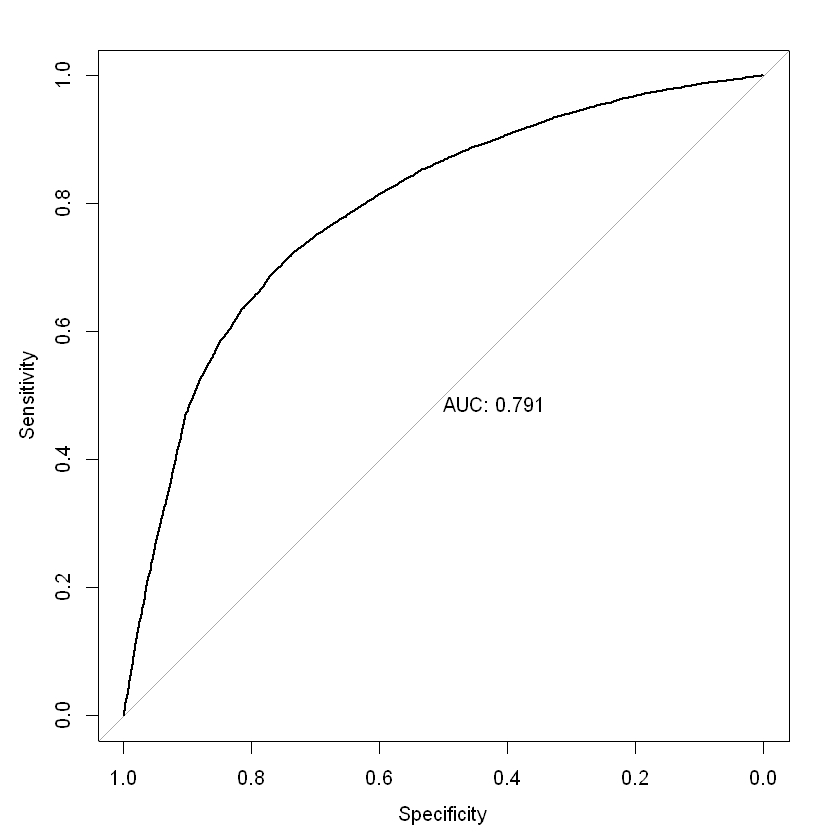
\includegraphics[width=\textwidth]{Images/roc1.png}
			\caption{Modelo 1}
		\end{minipage}
		\hspace{2mm}
		\begin{minipage}[b]{0.35\textwidth}
			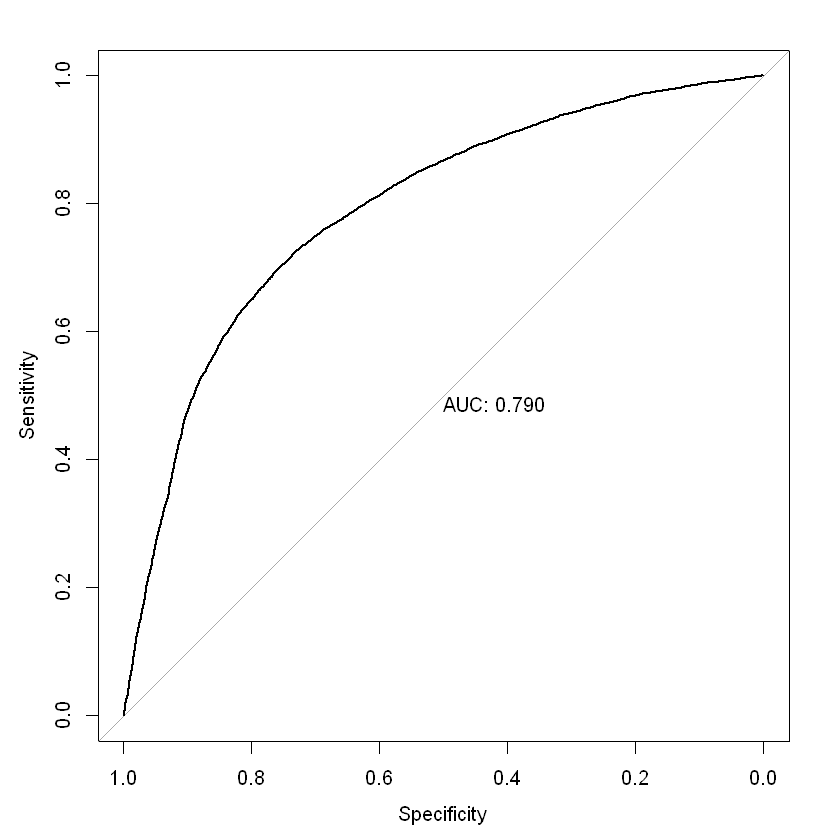
\includegraphics[width=\textwidth]{Images/roc2.png}
			\caption{Modelo 2}
		\end{minipage}
	\end{figure}

	% ---
	% Finaliza a parte no bookmark do PDF, para que se inicie o bookmark na raiz
	% ---
	
	% ---
	% Conclusão
	% ---
	\section{Discussão}
	Através da nossa pesquisa, aprendemos que variáveis como idade, IMC, peso, pressão sistólica, diastólica e níveis de colesterol são significantemente correlacionados com o risco de desenvolver doenças cardiovasculares. Esses resultados confirmam descobertas prévias na área da cardiologia, como foi mencionado na introdução.
	
	Ao testar nossos modelos para calcular a probabilidade em grupos específicos como pessoas entre 50-60 do grupo de teste e obter os valores reais do grupo de treino, obtive resultados próximos, sendo eles 0.5325 para os modelos e 0.5190 a probabilidade real.  Para outras faixas etárias, também obtive o mesmo efeito, quando pessoas tinham entre 30-40 anos o modelo previa 0.31 dada 0.33 a probabilidade real.
	
	Apesar de tentar métodos alternativos como a função LinearRegression() do pacote \textit{Scikit-Learn} em Python ou a função cv.glmnet() do pacote \textit{glmnet} em R, as métricas obtidas foram praticamente as mesmas dos nossos modelos em GLM, com acurácia em torno de 70-72\%. Com isso, podemos dizer que foi alcançado o objetivo de identificar os fatores que possuem maior
	influência da doenças cardiovasculares, mas não um modelo aceitável para a aplicação na área da saúde.
	
	O GLM é um modelo linear, o que significa que ele pode não ser capaz de capturar relações complexas e não-lineares entre as variáveis. Além disso, a provável ausência de algumas variáveis importantes no nosso dataset pode ter levado a uma visão parcial do risco cardiovascular. Por exemplo, informações sobre a história familiar de doenças cardiovasculares, dieta \cite{cervato1997dieta} e estilo de vida dos indivíduos poderiam ter enriquecido nosso modelo. 
	
	De um ponto de vista metodológico, enfrentamos limitações relacionadas a nossa compreensão e aplicação de algoritmos de machine learning e validação cruzada. Embora tenhamos utilizado o modelo de Regressão Logística Generalizada (GLM), que é uma ferramenta robusta e amplamente usada, acreditamos que uma abordagem baseada em aprendizado de máquinas, como o uso de algoritmos mais sofisticados, tais como "random forest" ou "boosting" \cite{santos2022analise}, poderiam ter levado a resultados mais precisos. Esses algoritmos poderiam permitir que o modelo considerasse interações complexas entre as variáveis.
	

	Então, em termos de direções futuras, acreditamos que seria valioso explorar os algoritmos mencionados e tentar coletar dados que incluam mais fatores de risco cardiovascular. O uso de técnicas de validação cruzada para otimizar os ajustes do modelo seria uma área importante para futuras investigações.
	 
	 Apesar dessas limitações, acreditamos que nosso estudo fornece uma contribuição valiosa para a compreensão dos fatores de risco cardiovascular. 
	
	% ----------------------------------------------------------

	% Agradecimentos
	% ----------------------------------------------------------
	
	\section*{Agradecimentos}
	Ao professor de estatística Luiz Max pela disponibilidade e compromisso em nos ajudar a crescer como pesquisadores na área. Ao longo do curso, suas habilidades de ensino e paixão pelo assunto foram evidentes. Seus insights foram fundamentais para a condução adequada da elaboração e análise de modelos, assim como as técnicas apropriadas para interpretação dos resultados.
	% ----------------------------------------------------------
	% Referências bibliográficas
	% ----------------------------------------------------------
	%\bibliography{abntex2-modelo-references}
	
	\newpage
	\bibliographystyle{plain}
	\bibliography{bibliography.bib}

	



\end{document}